\documentclass[aip,jap,reprint,amsmath,amssymb,floatfix]{revtex4-2}
\usepackage{graphicx}
\usepackage{booktabs}
\usepackage{longtable}
\usepackage[hidelinks]{hyperref}
\usepackage{url}

\renewcommand{\thetable}{S\arabic{table}}
\renewcommand{\thefigure}{S\arabic{figure}}
\renewcommand{\theequation}{S\arabic{equation}}
\renewcommand{\thesection}{S\arabic{section}}

\begin{document}

\title{Supplementary Material for ``Special optimal thermal cells: D-optimal
thermal displacements for finite-temperature effective-harmonic phonons''}

\author{Albert Linda}
\affiliation{Department of Materials Science and Engineering, Indian Institute
of Technology Kanpur, Kanpur 208016, India}

\maketitle

\section{Surrogate design study}

Table~\ref{tab:surrogate} lists the median phonon-mesh errors of six
displacement designs on the DFT-fitted FC2+FC3+FC4 surrogates of Al, W, and
NaCl. The surrogate effective FC2 was fitted to 6000 paired canonical
samples; fitting half of them changes the mesh frequencies by 0.002 (Al),
0.001 (W), and 0.006~THz (NaCl). All designs were drawn from the harmonic FD
model of the same $3\times3\times3$ cell and fitted in the space-group adapted
FC2 basis with the cutoffs of the main text. Held-out forces on 200 canonical
configurations follow the same ordering.

\begin{table*}[t]
\caption{Surrogate design study (Al 300~K, W 1500~K, NaCl 700~K; DFT-fitted FC2+FC3+FC4 surrogates in $3\times3\times3$ cells). Median mesh RMSE (THz) against the surrogate effective FC2 over 30 repetitions, at 2/4/8/16 force calls.}
\label{tab:surrogate}
\begin{ruledtabular}
\begin{tabular}{lccc}
Design & Al & W & NaCl\\
\hline
Canonical & 0.199/0.123/0.088/0.064 & 0.091/0.068/0.048/0.033 & 0.224/0.185/0.116/0.089\\
Canonical $\pm$ & 0.066/0.054/0.038/0.032 & 0.035/0.027/0.021/0.018 & 0.176/0.127/0.078/0.078\\
Exact ampl., random signs & 0.066/0.050/0.038/0.025 & 0.035/0.028/0.017/0.016 & 0.166/0.131/0.093/0.063\\
SOTC-D & 0.063/0.056/0.040/0.025 & 0.039/0.024/0.021/0.015 & 0.150/0.131/0.090/0.062\\
Stratified ampl. + D-opt. & 0.073/0.046/0.038/0.028 & 0.035/0.031/0.020/0.015 & 0.151/0.134/0.088/0.089\\
Gaussian ampl. + D-opt. & 0.074/0.053/0.046/0.030 & 0.048/0.032/0.024/0.019 & 0.184/0.124/0.114/0.077\\
\hline
Harmonic vs effective & 0.229 & 0.149 & 0.765\\
\end{tabular}
\end{ruledtabular}
\end{table*}


\section{Designs in the crystal-symmetry basis}

Table~\ref{tab:selfconsistent_crystal} repeats Table~V of the main text with
all fits in the FC2 basis of the full crystal space group (hiPhive cluster
space, 3--12 parameters, cutoff limited to half the shortest image distance).
For Si and Mg the two bases coincide.

\begin{table*}[t]
\caption{Updated trial (iteration 1, crystal basis). Mesh RMSE (THz) against the iteration-1 effective FC2. Matched trial: SOTC-D designed from the iteration-1 trial (D$_1$) versus the better of random canonical subsets and pairs drawn from the same trial (C$_1$), scored against the disjoint effective FC2. Equal cost: bootstrapped SOTC-D (B; first pair from the harmonic trial, later pairs from the model refitted to the first pair, no extra force calls) and one-shot SOTC-D (D$_0$) versus canonical pairs from the harmonic trial (C$_0$; a single sTDEP iteration), scored against the 40-snapshot iteration-1 effective FC2, which shares no configuration with them. B and D$_0$ coincide at 2 calls by construction. The best entry of each group is bold.}
\label{tab:selfconsistent_crystal}
\begin{ruledtabular}
\begin{tabular}{lcccccccccc}
 & \multicolumn{2}{c}{matched, 2} & \multicolumn{3}{c}{equal cost, 2} & \multicolumn{2}{c}{matched, 8} & \multicolumn{3}{c}{equal cost, 8}\\
 & D$_1$ & C$_1$ & B & D$_0$ & C$_0$ & D$_1$ & C$_1$ & B & D$_0$ & C$_0$\\
\hline
Al & \textbf{0.06} & 0.08 & \textbf{0.07} & 0.07 & 0.10 & \textbf{0.03} & 0.05 & \textbf{0.03} & 0.05 & 0.04\\
Ag & \textbf{0.04} & 0.11 & \textbf{0.02} & 0.02 & 0.13 & 0.06 & \textbf{0.05} & \textbf{0.06} & 0.09 & 0.10\\
Au & 0.08 & \textbf{0.08} & \textbf{0.15} & 0.15 & 0.24 & \textbf{0.05} & 0.05 & \textbf{0.02} & 0.17 & 0.22\\
Cu & \textbf{0.08} & 0.15 & 0.20 & 0.20 & \textbf{0.07} & \textbf{0.04} & 0.08 & 0.17 & \textbf{0.10} & 0.14\\
Mo & 0.06 & \textbf{0.06} & \textbf{0.05} & 0.05 & 0.07 & \textbf{0.02} & 0.03 & \textbf{0.02} & 0.03 & 0.06\\
W & 0.05 & \textbf{0.04} & 0.05 & 0.05 & \textbf{0.04} & \textbf{0.02} & 0.02 & 0.02 & \textbf{0.02} & 0.02\\
NaCl & \textbf{0.05} & 0.11 & \textbf{0.11} & 0.11 & 0.14 & 0.09 & \textbf{0.07} & \textbf{0.05} & 0.15 & 0.12\\
MgO & \textbf{0.22} & 0.32 & 0.42 & 0.42 & \textbf{0.34} & \textbf{0.09} & 0.15 & \textbf{0.11} & 0.32 & 0.26\\
PbTe & \textbf{0.02} & 0.07 & 0.19 & 0.19 & \textbf{0.13} & \textbf{0.02} & 0.03 & \textbf{0.03} & 0.12 & 0.09\\
Si & \textbf{0.07} & 0.10 & \textbf{0.10} & 0.10 & 0.11 & \textbf{0.05} & 0.05 & \textbf{0.05} & 0.09 & 0.07\\
Mg & \textbf{0.05} & 0.06 & \textbf{0.06} & 0.06 & 0.07 & \textbf{0.03} & 0.05 & \textbf{0.02} & 0.06 & 0.04\\
\hline
D$_1<$C$_1$ / B$<$C$_0$ & \multicolumn{2}{c}{8/11} & \multicolumn{3}{c}{7/11} & \multicolumn{2}{c}{9/11} & \multicolumn{3}{c}{9/11}\\
held-out force D$_1<$C$_1$ & \multicolumn{2}{c}{9/11} & \multicolumn{3}{c}{} & \multicolumn{2}{c}{8/11} & \multicolumn{3}{c}{}\\
\end{tabular}
\end{ruledtabular}
\end{table*}


Table~\ref{tab:stdep_crystal} repeats the DFT sTDEP comparison of the main
text in the crystal-symmetry basis.

\begin{table*}[t]
\caption{Self-consistent protocols with DFT forces, equal cost. Mesh RMSE (THz) against the 40-snapshot iteration-1 effective FC2 (crystal basis). B: bootstrapped SOTC-D. sTDEP: half of the calls as canonical $\pm$ pairs from the harmonic trial, half as canonical $\pm$ pairs from the model refitted to them, fitted to the second iteration only (last) or to both (pool); median of three seeds. C$_0$: one-shot canonical pairs from the harmonic trial (median of 20 subsets). No configuration of any protocol enters the reference. The best entry of each group is bold.}
\label{tab:stdep_crystal}
\begin{ruledtabular}
\begin{tabular}{lcccccccc}
 & \multicolumn{4}{c}{8 calls} & \multicolumn{4}{c}{16 calls}\\
 & B & sTDEP last & sTDEP pool & C$_0$ & B & sTDEP last & sTDEP pool & C$_0$\\
\hline
Al & \textbf{0.03} & 0.05 & 0.05 & 0.04 & 0.02 & 0.03 & \textbf{0.01} & 0.03\\
Ag & 0.06 & \textbf{0.04} & 0.07 & 0.10 & 0.04 & \textbf{0.03} & 0.09 & 0.10\\
Au & \textbf{0.02} & 0.06 & 0.17 & 0.22 & \textbf{0.01} & 0.04 & 0.15 & 0.21\\
Cu & 0.17 & 0.18 & \textbf{0.10} & 0.14 & 0.16 & 0.08 & \textbf{0.06} & 0.14\\
Mo & \textbf{0.02} & 0.05 & 0.03 & 0.06 & 0.02 & 0.03 & \textbf{0.02} & 0.05\\
W & 0.02 & 0.05 & 0.03 & \textbf{0.02} & 0.02 & 0.03 & \textbf{0.02} & 0.02\\
NaCl & \textbf{0.05} & 0.13 & 0.09 & 0.12 & \textbf{0.04} & 0.10 & 0.13 & 0.12\\
MgO & \textbf{0.11} & 0.22 & 0.18 & 0.26 & \textbf{0.10} & 0.19 & 0.22 & 0.25\\
PbTe & \textbf{0.03} & 0.05 & 0.07 & 0.09 & \textbf{0.04} & 0.04 & 0.06 & 0.08\\
Si & \textbf{0.05} & 0.08 & 0.08 & 0.07 & \textbf{0.04} & 0.05 & 0.06 & 0.06\\
Mg & \textbf{0.02} & 0.05 & 0.03 & 0.04 & \textbf{0.02} & 0.04 & 0.04 & 0.03\\
\hline
B best & \multicolumn{4}{c}{8/11} & \multicolumn{4}{c}{6/11}\\
\end{tabular}
\end{ruledtabular}
\end{table*}


\section{Regression frameworks}

Table~\ref{tab:fitters} compares nine regression methods of the trainstation
package, as used in hiPhive workflows, on the same DFT data and the same
crystal-symmetry cluster space. Hyperparameters were selected by the
package's internal cross-validation. All methods agree to within 0.03~THz.

\begin{table*}[t]
\caption{Regression frameworks (hiPhive cluster space with crystal symmetry, trainstation fit methods) on the same DFT data, 8 force calls. Entries: mesh RMSE (THz) against the disjoint effective FC2 (supercell basis, so the entries include the basis difference listed in the main text) for random canonical subsets (median of 10) / SOTC-D.}
\label{tab:fitters}
\footnotesize
\begin{ruledtabular}
\begin{tabular}{lccccccccccc}
Method & Al & Ag & Au & Cu & Mo & W & NaCl & MgO & PbTe & Si & Mg\\
\hline
least-squares & 0.20/0.18 & 0.11/0.09 & 0.12/0.13 & 0.23/0.20 & 0.09/0.08 & 0.06/0.05 & 0.13/0.11 & 0.31/0.26 & 0.06/0.11 & 0.10/0.05 & 0.08/0.04\\
ridge & 0.20/0.18 & 0.11/0.09 & 0.12/0.13 & 0.24/0.20 & 0.09/0.08 & 0.06/0.05 & 0.13/0.12 & 0.31/0.26 & 0.06/0.12 & 0.10/0.05 & 0.08/0.04\\
bayesian-ridge & 0.20/0.18 & 0.11/0.09 & 0.12/0.14 & 0.24/0.20 & 0.09/0.08 & 0.06/0.05 & 0.13/0.12 & 0.31/0.26 & 0.06/0.12 & 0.10/0.05 & 0.08/0.03\\
ardr & 0.20/0.18 & 0.11/0.09 & 0.12/0.14 & 0.24/0.20 & 0.09/0.08 & 0.06/0.05 & 0.14/0.11 & 0.32/0.27 & 0.07/0.12 & 0.08/0.06 & 0.07/0.04\\
rfe & 0.20/0.18 & 0.11/0.09 & 0.12/0.13 & 0.23/0.20 & 0.09/0.08 & 0.06/0.05 & 0.13/0.11 & 0.33/0.26 & 0.06/0.12 & 0.10/0.07 & 0.07/0.04\\
omp & 0.20/0.18 & 0.11/0.09 & 0.12/0.13 & 0.23/0.20 & 0.09/0.08 & 0.06/0.05 & 0.14/0.11 & 0.31/0.26 & 0.06/0.11 & 0.10/0.08 & 0.07/0.04\\
lasso & 0.20/0.18 & 0.11/0.09 & 0.12/0.13 & 0.23/0.20 & 0.09/0.08 & 0.06/0.05 & 0.14/0.11 & 0.31/0.26 & 0.06/0.11 & 0.09/0.06 & 0.07/0.04\\
adaptive-lasso & 0.20/0.18 & 0.13/0.12 & 0.12/0.16 & 0.23/0.20 & 0.09/0.08 & 0.06/0.05 & 0.14/0.11 & 0.31/0.26 & 0.06/0.11 & 0.09/0.05 & 0.08/0.06\\
elasticnet & 0.20/0.18 & 0.11/0.09 & 0.12/0.13 & 0.23/0.20 & 0.09/0.08 & 0.06/0.05 & 0.14/0.11 & 0.31/0.26 & 0.06/0.11 & 0.09/0.06 & 0.07/0.04\\
\end{tabular}
\end{ruledtabular}
\end{table*}


\section{Derivations for the estimator theory}

\textit{Effective FC2 as averaged Hessian.} For $\mathbf u\sim
N(\mathbf 0,\mathbf C)$ and smooth $V$, Stein's lemma states
$\langle\mathbf u\,g(\mathbf u)\rangle=\mathbf C\langle\nabla g\rangle$.
With $g=\mathbf F^{\rm T}=-\nabla V^{\rm T}$ this gives
$\langle\mathbf u\mathbf F^{\rm T}\rangle=-\mathbf C\langle\nabla\nabla V\rangle$,
so the population least-squares coefficient of $\mathbf F$ on $\mathbf u$ is
$-\langle\mathbf F\mathbf u^{\rm T}\rangle\mathbf C^{-1}=\langle\nabla\nabla V\rangle$.
The SCHA free-energy gradient with respect to the auxiliary FC2 vanishes
when $\langle\nabla\nabla V\rangle_{\mathbf C(\boldsymbol\Phi)}=\boldsymbol\Phi$
for a fixed centroid, which is the self-consistent fixed point of the main
text.

\textit{Fixed-amplitude bias.} In mass-weighted normal coordinates with
forces $f_a=-\omega_a^2Q_a-\tfrac12V_{abc}Q_bQ_c-\tfrac16V_{abcd}Q_bQ_cQ_d$,
the regression coefficient for a design with independent symmetric
coordinates is $\Phi_{ae}=-\langle f_aQ_e\rangle/\langle Q_e^2\rangle$. The
cubic term vanishes by symmetry. The quartic term needs
$\langle Q_bQ_cQ_dQ_e\rangle$, which for distinct indices paired as
$(bb)(ee)$ equals $\sigma_b^2\sigma_e^2$ for both Gaussian and $\pm\sigma$
coordinates, and for $b=c=d=e$ equals $3\sigma_e^4$ (Gaussian) or
$\sigma_e^4$ (fixed amplitude). Collecting the three pairings,
\begin{equation}
\Phi_{ae}=\omega_a^2\delta_{ae}+\tfrac12\sum_{b}V_{abbe}\sigma_b^2
-\tfrac{1}{6}\,(3-\kappa_e)\,V_{aeee}\sigma_e^2,
\end{equation}
with $\kappa_e=\langle Q_e^4\rangle/\sigma_e^4$. The last term vanishes for
Gaussian coordinates ($\kappa_e=3$) and equals $-\tfrac13V_{aeee}\sigma_e^2$ for
the fixed-amplitude design ($\kappa_e=1$). The
statement is verified numerically by exact enumeration of all $2^6$ sign
patterns of a random six-mode quartic model in the test suite
(\texttt{test\_optimal\_design.py}), as are the exact cancellation of
arbitrary cubic forces by $\pm$ pairs and the thermal mean-square
displacements of the ZG and rattle designs.

\section{Higher-order force-constant validation}

Figure~\ref{fig:ifc34} documents the joint FC2+FC3+FC4 fits used as
surrogates: held-out errors of the nested models, convergence with the number
of training snapshots, sensitivity to the interaction cutoffs, and comparison
with the force changes produced by higher plane-wave cutoffs and denser $k$
meshes. For Al the denser-$k$-mesh force change exceeds the final fit error,
so the Al tensors are used here only as model potentials for the
sampling study, not as converged inputs for transport calculations.

\begin{figure*}[t]
\centering
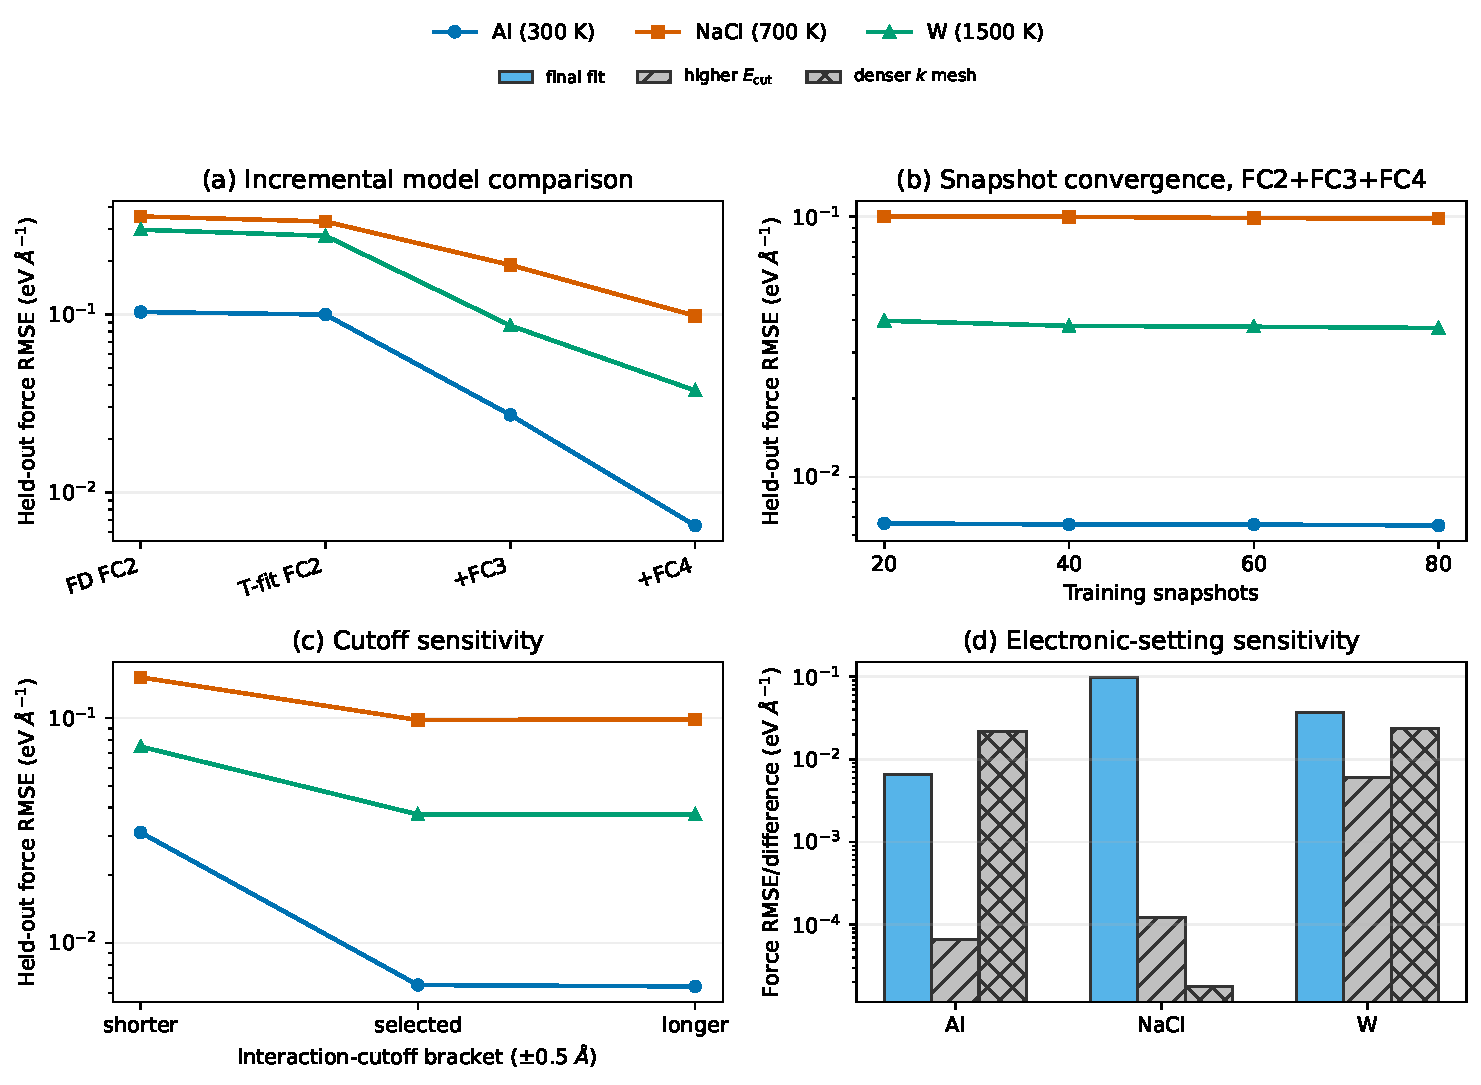
\includegraphics[width=0.95\textwidth]{figures/fig_ifc34_diagnostics.pdf}
\caption{Validation of the FC2+FC3+FC4 fits to 80 canonical QE snapshots
(Al 300~K, W 1500~K, NaCl 700~K; $3\times3\times3$ cells). (a) Held-out force
RMSE of harmonic FD FC2 and of temperature-fitted FC2, FC2+FC3, and
FC2+FC3+FC4 models. (b) Convergence with training snapshots. (c) Cutoff
sensitivity ($\pm0.5$~\AA). (d) Fit error compared with electronic-setting
force differences.}
\label{fig:ifc34}
\end{figure*}

\clearpage
\section{Individual iterations of the SOTC-C runs}

\begin{longtable*}{lcccccc}
\caption{Individual iterations of the SOTC-C runs: configurations, rms displacement, unstable mesh fraction and minimum frequency of the axial-prior fit, and normalized condition number of the space-group adapted design.\label{tab:iterations}}\\
\hline\hline
Material & iter. & $N_{\rm ens}$ & $u_{\rm rms}$ (\AA) & $f_{\rm unst}$ & $\omega_{\min}$ (THz) & cond.\\
\hline
\endfirsthead
\hline
Material & iter. & $N_{\rm ens}$ & $u_{\rm rms}$ (\AA) & $f_{\rm unst}$ & $\omega_{\min}$ (THz) & cond.\\
\hline
\endhead
Al & 1 & 5 & 0.106 & 0.000 & 0.60 & 5.2\\
Al & 2* & 5 & 0.106 & 0.000 & 0.48 & 3.4\\
Ag & 1 & 5 & 0.167 & 0.000 & 0.26 & 5.7\\
Ag & 2 & 5 & 0.167 & 0.000 & 0.42 & 3.2\\
Ag & 3 & 5 & 0.167 & 0.000 & 0.44 & 3.2\\
Ag & 4* & 5 & 0.167 & 0.000 & 0.32 & 2.8\\
Au & 1* & 1 & 0.186 & 0.007 & -0.95 & 10.7\\
Au & 2 & 1 & 0.186 & 0.159 & -4.58 & 7.5\\
Cu & 1 & 8 & 0.169 & 0.000 & 0.51 & 15.3\\
Cu & 2 & 8 & 0.169 & 0.000 & 0.45 & 7.9\\
Cu & 3* & 8 & 0.169 & 0.000 & 0.45 & 7.5\\
Cu & 4 & 8 & 0.169 & 0.000 & 0.52 & 8.2\\
Mo & 1 & 1 & 0.111 & 0.000 & 0.52 & 17.1\\
Mo & 2* & 1 & 0.111 & 0.000 & 0.99 & 8.0\\
W & 1 & 3 & 0.115 & 0.000 & 0.76 & 4.5\\
W & 2* & 3 & 0.115 & 0.000 & 0.73 & 2.9\\
W & 3 & 3 & 0.115 & 0.000 & 0.75 & 3.5\\
W & 4 & 3 & 0.115 & 0.000 & 0.74 & 3.3\\
NaCl & 1 & 3 & 0.191 & 0.000 & 0.31 & 3.9\\
NaCl & 2 & 3 & 0.191 & 0.000 & 0.34 & 2.8\\
NaCl & 3 & 3 & 0.191 & 0.000 & 0.32 & 2.9\\
NaCl & 4 & 3 & 0.191 & 0.000 & 0.39 & 3.1\\
NaCl & 5* & 3 & 0.191 & 0.000 & 0.31 & 2.4\\
MgO & 1 & 3 & 0.141 & 0.000 & 0.96 & 2.9\\
MgO & 2 & 3 & 0.141 & 0.000 & 0.73 & 2.1\\
MgO & 3 & 3 & 0.141 & 0.000 & 0.96 & 2.6\\
MgO & 4* & 3 & 0.141 & 0.000 & 0.88 & 2.2\\
PbTe & 1 & 5 & 0.190 & 0.000 & 0.21 & 3.1\\
PbTe & 2* & 5 & 0.190 & 0.000 & 0.22 & 2.2\\
PbTe & 3 & 5 & 0.190 & 0.000 & 0.19 & 2.1\\
PbTe & 4 & 5 & 0.190 & 0.000 & 0.22 & 2.4\\
\hline\hline
\end{longtable*}


\noindent An asterisk marks the iteration selected by the workflow.
The two Au iterations each contain a single configuration; their
axial-prior fits are unstable, whereas the pooled fit is stable.

\section{Lattice-parameter sensitivity}

\begin{table*}[t]
\caption{PBE equilibrium lattice parameters from Birch--Murnaghan fits (primitive cells) and the effect of using them instead of the production values on the harmonic $3\times3\times3$ FD model: mesh RMSE and change in $S_{\rm vib}(T_{\rm des})$.}
\label{tab:volume}
\begin{ruledtabular}
\begin{tabular}{lcccccc}
 & $a_{\rm prod}$ (\AA) & $a_{\rm PBE}$ (\AA) & $\Delta a/a$ (\%) & $B_0$ (GPa) & RMSE (THz) & $\Delta S_{\rm vib}$\\
\hline
Al & 4.050 & 4.039 & -0.26 & 78 & 0.10 & -0.38\\
Ag & 4.120 & 4.146 & +0.63 & 91 & 0.16 & +1.17\\
Au & 4.130 & 4.150 & +0.49 & 142 & 0.12 & +1.17\\
Cu & 3.670 & 3.631 & -1.06 & 142 & 0.35 & -1.71\\
Mo & 3.160 & 3.160 & -0.01 & 259 & 0.00 & -0.01\\
W & 3.180 & 3.184 & +0.14 & 305 & 0.03 & +0.18\\
NaCl & 5.730 & 5.704 & -0.45 & 24 & 0.12 & -0.64\\
MgO & 4.260 & 4.249 & -0.25 & 153 & 0.14 & -0.30\\
PbTe & 6.510 & 6.567 & +0.88 & 39 & 0.14 & +1.72\\
\end{tabular}
\end{ruledtabular}
\end{table*}


\section{Accuracy overview}

\begin{figure*}[t]
\centering
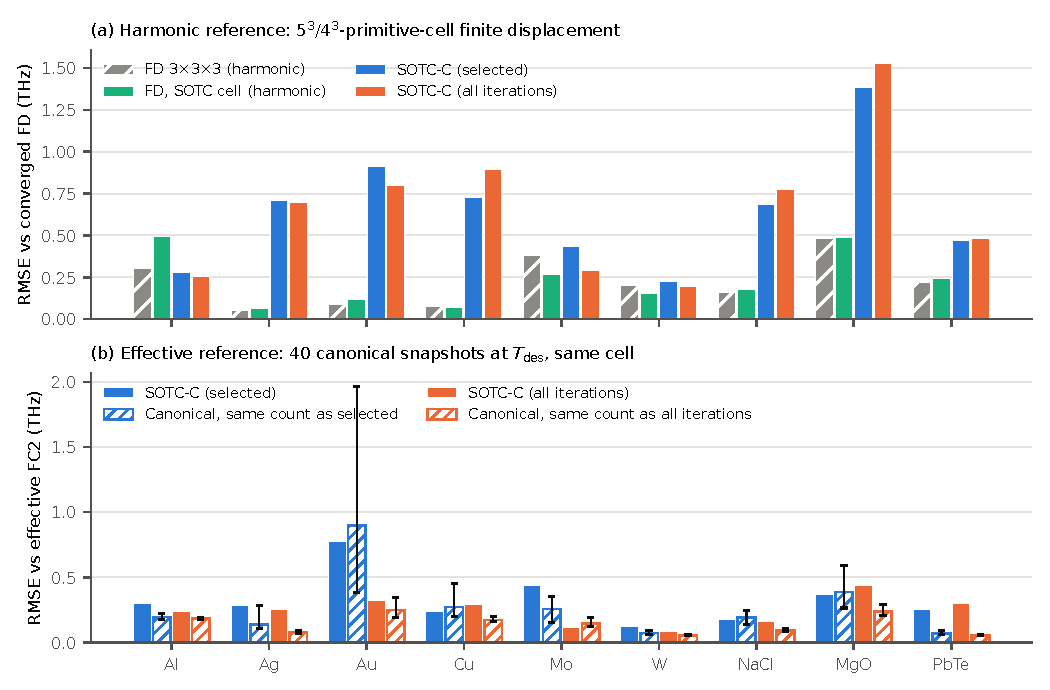
\includegraphics[width=\textwidth]{figures/fig_reference_accuracy.pdf}
\caption{(a) Mesh RMSE against the converged large-cell harmonic FD reference
for harmonic FD in $3\times3\times3$ cells and in the SOTC cells, and for the
selected and pooled SOTC-C models. (b) Mesh RMSE against the same-cell
effective FC2 for the selected and pooled SOTC-C models and for random
canonical subsets of the same size fitted with the same prior (median and
10--90\% range over 20 draws).}
\label{fig:accuracy}
\end{figure*}

\section{NaCl optic modes and neutron data}

\begin{figure*}[t]
\centering
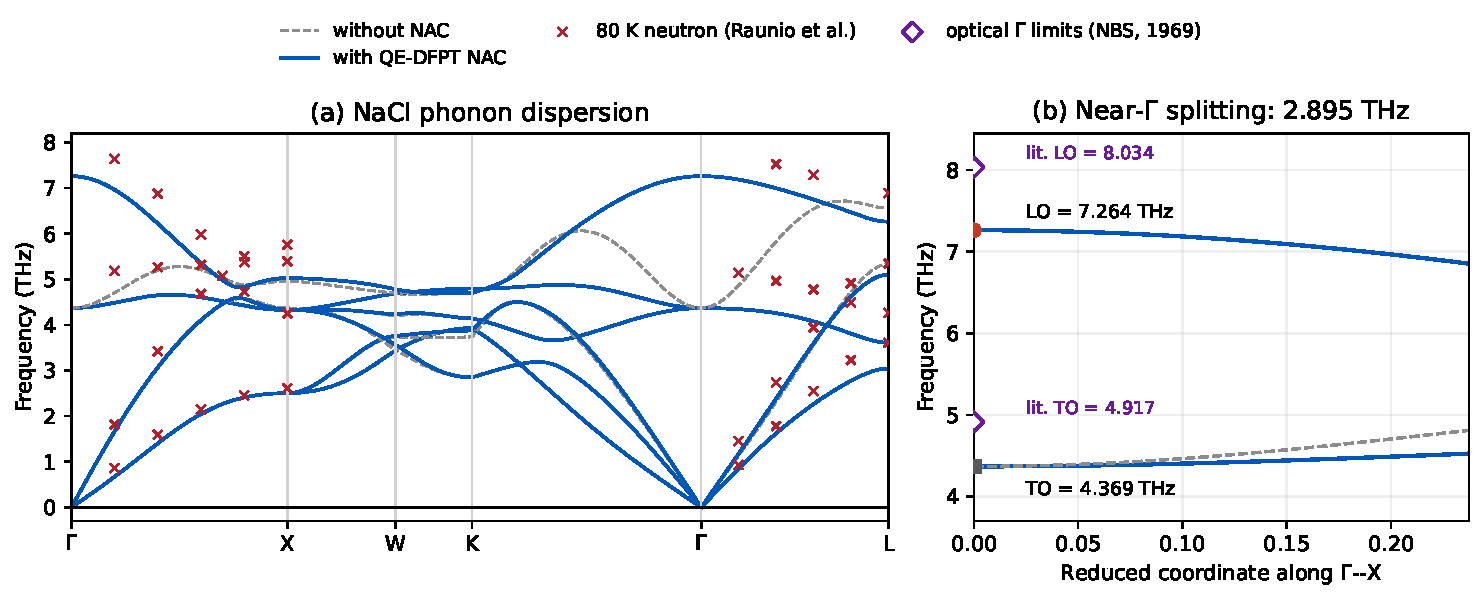
\includegraphics[width=0.95\textwidth]{figures/fig_nacl_loto.pdf}
\caption{NaCl harmonic FD FC2 ($3\times3\times3$ cell) without (gray dashed)
and with (blue) the non-analytic correction from QE-DFPT Born charges and
dielectric tensor. Red crosses: 39 neutron points at 80~K along $\Gamma$--X
and $\Gamma$--L \cite{ref35}; purple diamonds: infrared TO and LO limits
\cite{ref48}. The neutron data are temperature-mismatched to the
fixed-volume calculation and are shown without a global error metric.}
\label{fig:nacl}
\end{figure*}

\section{Thermal displacement correlator}

In second quantization, the displacement of basis atom $a$ in cell
$\mathbf R$ is
\begin{equation}
\hat u_a^\alpha(\mathbf R)=\frac{1}{\sqrt{N_c}}\sum_{\mathbf qs}
\sqrt{\frac{\hbar}{2M_a\omega_{\mathbf qs}}}\,e_a^\alpha(\mathbf qs)
\left(\hat a_{\mathbf qs}+\hat a^\dagger_{-\mathbf qs}\right)
e^{i\mathbf q\cdot\mathbf R}.
\end{equation}
With $\langle\hat a^\dagger_{\mathbf qs}\hat a_{\mathbf q's'}\rangle=n_B\delta\delta$,
$\langle\hat a_{\mathbf qs}\hat a^\dagger_{\mathbf q's'}\rangle=(n_B+1)\delta\delta$,
vanishing anomalous averages, and $2n_B+1=\coth(\hbar\omega/2k_BT)$,
the canonical average $\langle\hat u_a^\alpha(\mathbf 0)\hat u_b^\beta(\mathbf R)\rangle$
reduces to Eq.~(4) of the main text: only $\mathbf q'=-\mathbf q$ contributes,
and $e^{\beta}_b(-\mathbf qs)=e^{\beta*}_b(\mathbf qs)$ gives the factor
$e^\alpha_a(\mathbf qs)e^{\beta*}_b(\mathbf qs)e^{-i\mathbf q\cdot\mathbf R}$. Its trace with the
completeness relation of the polarization vectors gives
$U_{\rm iso}=(\hbar/6N_cM)\sum_{\mathbf qs}\omega_{\mathbf qs}^{-1}
\coth(\hbar\omega_{\mathbf qs}/2k_BT)$ for a monatomic crystal.

In the commensurate supercell the same covariance is diagonal in the
normal-mode coordinates $Q_m$ with variances $\sigma_m^2$ given in Sec.~II~D
of the main text. A configuration of the form of Eq.~(7) has
$Q_m^2=\sigma_m^2$ for every mode, so that its single-configuration
second moment equals the canonical one mode by mode; cross terms
$Q_mQ_{m'}=s_ms_{m'}\sigma_m\sigma_{m'}$ average to zero only over the
sign patterns, and their effect on the force fit is what the D-optimal sign
choice controls.

\section{SOTC objective gradient}

For the shell objective of Eq.~(6) of the main text, write the cell
correlator as a sum over ordered atom pairs,
$\bar C_{2,ab}^{\rm cell}(R;\mathbf u)=\sum_{i,j}P^{abR}_{ij}\,\mathbf u_i\cdot\mathbf u_j$,
where the symmetric weight matrix $P^{abR}_{ij}$ equals $1/(3N_R^{ab}N_a)$ (or half
of it for each order when $a\neq b$) if the pair belongs to shell $R$ of the
species channel and zero otherwise; the on-site term is the shell $R=0$. Then
\begin{equation}
\frac{\partial\mathcal Q}{\partial\mathbf u_i}=
\sum_{a,b,R}4\,w_{ab}(R)\,\Delta_{ab}(R)\sum_jP^{abR}_{ij}\,\mathbf u_j ,
\end{equation}
with $\Delta_{ab}(R)=\bar C_{2,ab}^{\rm cell}-\bar C_{2,ab}$, and the
mode-amplitude gradient follows by the chain rule through
$\mathbf u_i=\sum_m A_m\mathbf e_{im}/\sqrt{M_i}$. The optimization is
carried out in mode amplitudes and phases with random restarts.

\section{Branch-resolved convergence and neutron model for Al}

Figure~\ref{fig:dispconv} shows the dispersions of SOTC-D from the updated
trial with 2, 4, 8, and 16 force calls for Al (300~K) and Au (1200~K),
together with the converged large-cell harmonic FD reference and the
40-snapshot iteration-1 effective FC2 of the same cell. For Au, whose
single-configuration SOTC-C fits are unstable (Table~\ref{tab:iterations}),
the SOTC-D dispersions are stable at every budget and approach the effective
FC2 branch by branch; with two calls the largest deviations are in the
transverse branches along X--W--K and $\Gamma$--L. For Al the Born--von
K\'arm\'an models fitted to the inelastic neutron spectrum at 10 and 300~K
\cite{kresch2008} (eight shells) are also shown. The converged harmonic reference agrees with the 10~K
model within 1.1\% at X and L. The 300~K model is softer in the transverse
branches (TA(X) 5.39~THz) than both the converged harmonic reference
(5.72~THz) and the effective FC2 of the 32-atom cell (6.01 and 6.29~THz, the
degeneracy being lifted by the cell), most of whose stiffening is already
present in the harmonic FD model of that cell (5.87 and 6.09~THz). A
quantitative test of the finite-temperature renormalization against
experiment is therefore limited by the supercell truncation of the
32-atom cell and by the non-uniqueness of density-of-states-fitted
force-constant models for individual branches, especially away from the
high-symmetry points.

\begin{figure*}[p]
\centering
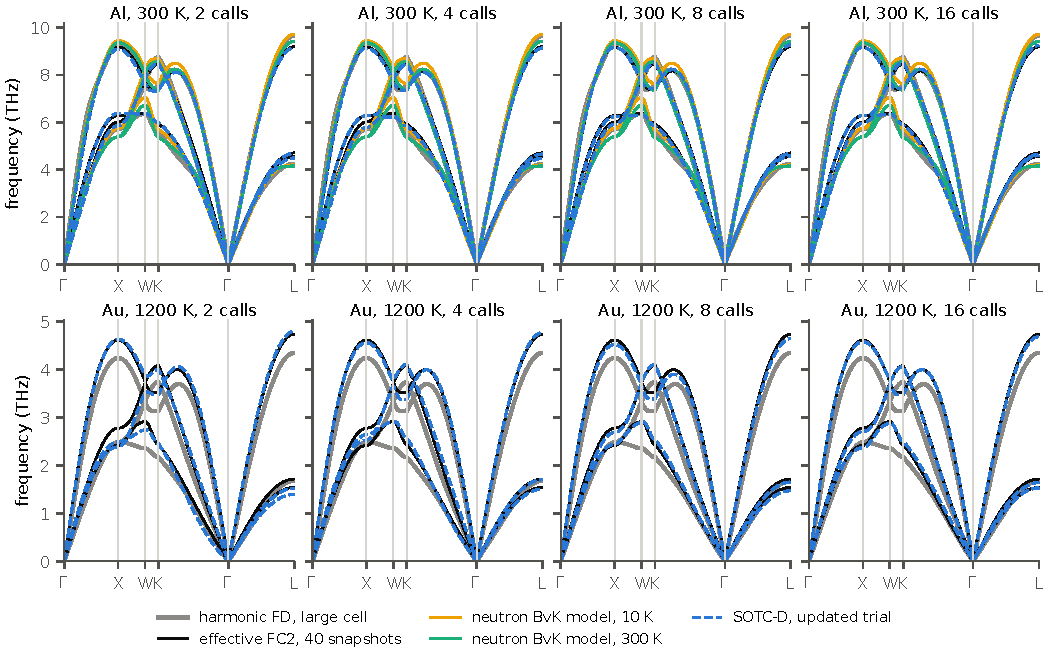
\includegraphics[width=\textwidth]{figures/fig_dispersion_convergence.pdf}
\caption{Dispersions of SOTC-D from the updated trial (blue dashed) with 2,
4, 8, and 16 force calls, the converged large-cell harmonic FD reference
(gray), the 40-snapshot iteration-1 effective FC2 (black), and, for Al, the
Born--von K\'arm\'an models fitted to inelastic neutron data at 10~K (yellow)
and 300~K (green). Same-cell models are Fourier interpolated from the
32-atom SOTC cell.}
\label{fig:dispconv}
\end{figure*}

\section{Designs at four and sixteen force calls}

Tables~\ref{tab:matched_4_16}, \ref{tab:selfconsistent_crystal_4_16}, and
\ref{tab:selfconsistent_4_16} extend Tables~IV and V of the main text and
Table~\ref{tab:selfconsistent_crystal} to four and sixteen force calls, with
the same definitions.

\begin{table*}[t]
\caption{Matched comparison in the SOTC cell at equal numbers of displaced force calls, all designed from the same-cell harmonic FD trial and fitted in the supercell space-group basis. D: SOTC-D; C: random canonical subsets; P: random canonical $\pm\mathbf u$ pairs (medians over 20 draws); Z: special displacements with Walsh sign patterns (ZG); R: thermal rattle (independent Gaussian atoms with the canonical per-atom variance). Upper block: held-out force RMSE on 8 canonical test snapshots relative to that of the 40-snapshot effective FC2. Lower block: mesh RMSE (THz) against an effective FC2 fitted to $40-n$ canonical snapshots disjoint from the scored design. The best entry is bold; the last row counts the materials in which D is best. Entries $>$10~THz ($>$100 in force) are singular fits of designs that do not identify the model.}
\label{tab:matched_4_16}
\begin{ruledtabular}
\begin{tabular}{lcccccccccc}
 & \multicolumn{5}{c}{4 calls} & \multicolumn{5}{c}{16 calls}\\
 & D & C & P & Z & R & D & C & P & Z & R\\
\hline
\multicolumn{11}{l}{Held-out force RMSE / floor}\\
Al & \textbf{1.005} & 1.053 & 1.015 & 1.025 & 1.050 & \textbf{0.997} & 1.007 & 1.001 & 1.020 & 1.019\\
Ag & \textbf{1.000} & 1.061 & 1.029 & 1.032 & 1.107 & \textbf{0.997} & 1.011 & 1.009 & 1.016 & 1.060\\
Au & \textbf{1.004} & 1.048 & 1.024 & 1.034 & 1.130 & \textbf{1.002} & 1.010 & 1.005 & 1.020 & 1.110\\
Cu & \textbf{1.038} & 1.154 & 1.186 & 1.567 & 1.366 & \textbf{1.006} & 1.032 & 1.013 & 1.026 & 1.073\\
Mo & \textbf{1.006} & 1.071 & 1.023 & 1.021 & 1.040 & \textbf{0.999} & 1.011 & 1.003 & 1.018 & 1.010\\
W & \textbf{1.007} & 1.057 & 1.017 & 1.026 & 1.024 & \textbf{0.997} & 1.010 & 1.002 & 1.010 & 1.005\\
NaCl & 1.005 & 1.005 & 1.005 & 1.002 & \textbf{0.996} & 1.002 & 1.001 & 1.000 & 0.999 & \textbf{0.982}\\
MgO & \textbf{1.012} & 1.035 & 1.031 & 1.030 & 1.135 & \textbf{0.998} & 1.007 & 1.005 & 1.005 & 1.058\\
PbTe & 1.027 & 1.018 & 1.018 & \textbf{1.011} & 1.045 & 1.012 & 1.003 & \textbf{1.001} & 1.016 & 1.141\\
Si & \textbf{0.999} & 1.005 & 1.002 & 1.001 & 1.131 & \textbf{0.998} & 1.002 & 1.000 & 1.000 & 1.116\\
Mg & \textbf{1.000} & 1.007 & 1.002 & 1.002 & 1.023 & 1.000 & 1.001 & 1.000 & \textbf{1.000} & 1.016\\
D best & \multicolumn{5}{c}{9/11} & \multicolumn{5}{c}{8/11}\\
\hline
\multicolumn{11}{l}{Mesh RMSE vs disjoint effective FC2 (THz)}\\
Al & \textbf{0.11} & 0.25 & 0.14 & 0.15 & 0.27 & \textbf{0.08} & 0.14 & 0.10 & 0.12 & 0.19\\
Ag & \textbf{0.11} & 0.32 & 0.21 & 0.24 & 0.41 & \textbf{0.10} & 0.18 & 0.14 & 0.18 & 0.30\\
Au & \textbf{0.17} & 0.27 & 0.20 & 0.30 & 0.40 & \textbf{0.11} & 0.17 & 0.13 & 0.19 & 0.42\\
Cu & \textbf{0.40} & 0.78 & 0.92 & 2.68 & 1.78 & 0.29 & 0.36 & \textbf{0.28} & 0.38 & 0.51\\
Mo & \textbf{0.08} & 0.17 & 0.10 & 0.11 & 0.14 & 0.06 & 0.11 & \textbf{0.05} & 0.11 & 0.10\\
W & \textbf{0.06} & 0.13 & 0.07 & 0.09 & 0.08 & \textbf{0.04} & 0.07 & 0.04 & 0.06 & 0.06\\
NaCl & 0.25 & 0.29 & \textbf{0.24} & 0.34 & 0.59 & 0.15 & 0.17 & \textbf{0.14} & 0.15 & 0.66\\
MgO & \textbf{0.40} & 0.57 & 0.52 & 0.47 & 1.05 & 0.34 & 0.39 & \textbf{0.30} & 0.36 & 0.74\\
PbTe & 0.16 & 0.13 & 0.13 & \textbf{0.12} & 0.27 & 0.10 & \textbf{0.08} & 0.08 & 0.09 & 0.37\\
Si & 0.04 & 0.12 & 0.07 & \textbf{0.03} & 0.62 & 0.04 & 0.07 & 0.04 & \textbf{0.04} & 0.56\\
Mg & \textbf{0.03} & 0.10 & 0.05 & 0.04 & 0.21 & 0.03 & 0.06 & \textbf{0.03} & 0.05 & 0.18\\
D best & \multicolumn{5}{c}{8/11} & \multicolumn{5}{c}{4/11}\\
\end{tabular}
\end{ruledtabular}
\end{table*}

\begin{table*}[t]
\caption{Updated trial (iteration 1, crystal basis). Mesh RMSE (THz) against the iteration-1 effective FC2. Matched trial: SOTC-D designed from the iteration-1 trial (D$_1$) versus the better of random canonical subsets and pairs drawn from the same trial (C$_1$), scored against the disjoint effective FC2. Equal cost: bootstrapped SOTC-D (B; first pair from the harmonic trial, later pairs from the model refitted to the first pair, no extra force calls) and one-shot SOTC-D (D$_0$) versus canonical pairs from the harmonic trial (C$_0$; a single sTDEP iteration), scored against the 40-snapshot iteration-1 effective FC2, which shares no configuration with them. B and D$_0$ coincide at 2 calls by construction. The best entry of each group is bold.}
\label{tab:selfconsistent_crystal_4_16}
\begin{ruledtabular}
\begin{tabular}{lcccccccccc}
 & \multicolumn{2}{c}{matched, 4} & \multicolumn{3}{c}{equal cost, 4} & \multicolumn{2}{c}{matched, 16} & \multicolumn{3}{c}{equal cost, 16}\\
 & D$_1$ & C$_1$ & B & D$_0$ & C$_0$ & D$_1$ & C$_1$ & B & D$_0$ & C$_0$\\
\hline
Al & 0.07 & \textbf{0.06} & \textbf{0.02} & 0.06 & 0.06 & \textbf{0.03} & 0.04 & \textbf{0.02} & 0.02 & 0.03\\
Ag & \textbf{0.04} & 0.08 & 0.08 & \textbf{0.06} & 0.08 & 0.05 & \textbf{0.05} & \textbf{0.04} & 0.06 & 0.10\\
Au & \textbf{0.03} & 0.07 & \textbf{0.07} & 0.16 & 0.19 & \textbf{0.04} & 0.05 & \textbf{0.01} & 0.17 & 0.21\\
Cu & \textbf{0.04} & 0.14 & 0.24 & 0.14 & \textbf{0.08} & \textbf{0.03} & 0.06 & 0.16 & \textbf{0.10} & 0.14\\
Mo & \textbf{0.02} & 0.04 & 0.02 & \textbf{0.02} & 0.06 & \textbf{0.02} & 0.03 & \textbf{0.02} & 0.03 & 0.05\\
W & \textbf{0.03} & 0.03 & 0.03 & \textbf{0.03} & 0.03 & \textbf{0.02} & 0.02 & 0.02 & \textbf{0.01} & 0.02\\
NaCl & 0.09 & \textbf{0.08} & \textbf{0.07} & 0.21 & 0.15 & 0.07 & \textbf{0.06} & \textbf{0.04} & 0.14 & 0.12\\
MgO & \textbf{0.13} & 0.18 & \textbf{0.27} & 0.37 & 0.31 & \textbf{0.10} & 0.12 & \textbf{0.10} & 0.32 & 0.25\\
PbTe & \textbf{0.02} & 0.05 & \textbf{0.07} & 0.17 & 0.10 & \textbf{0.03} & 0.03 & \textbf{0.04} & 0.11 & 0.08\\
Si & \textbf{0.05} & 0.07 & \textbf{0.06} & 0.09 & 0.09 & 0.06 & \textbf{0.04} & \textbf{0.04} & 0.09 & 0.06\\
Mg & \textbf{0.04} & 0.05 & 0.03 & \textbf{0.03} & 0.04 & 0.04 & \textbf{0.04} & \textbf{0.02} & 0.04 & 0.03\\
\hline
D$_1<$C$_1$ / B$<$C$_0$ & \multicolumn{2}{c}{9/11} & \multicolumn{3}{c}{9/11} & \multicolumn{2}{c}{7/11} & \multicolumn{3}{c}{10/11}\\
\end{tabular}
\end{ruledtabular}
\end{table*}

\begin{table*}[t]
\caption{Updated trial (iteration 1, supercell basis). Mesh RMSE (THz) against the iteration-1 effective FC2. Matched trial: SOTC-D designed from the iteration-1 trial (D$_1$) versus the better of random canonical subsets and pairs drawn from the same trial (C$_1$), scored against the disjoint effective FC2. Equal cost: bootstrapped SOTC-D (B; first pair from the harmonic trial, later pairs from the model refitted to the first pair, no extra force calls) and one-shot SOTC-D (D$_0$) versus canonical pairs from the harmonic trial (C$_0$; a single sTDEP iteration), scored against the 40-snapshot iteration-1 effective FC2, which shares no configuration with them. B and D$_0$ coincide at 2 calls by construction. The best entry of each group is bold.}
\label{tab:selfconsistent_4_16}
\begin{ruledtabular}
\begin{tabular}{lcccccccccc}
 & \multicolumn{2}{c}{matched, 4} & \multicolumn{3}{c}{equal cost, 4} & \multicolumn{2}{c}{matched, 16} & \multicolumn{3}{c}{equal cost, 16}\\
 & D$_1$ & C$_1$ & B & D$_0$ & C$_0$ & D$_1$ & C$_1$ & B & D$_0$ & C$_0$\\
\hline
Al & \textbf{0.10} & 0.21 & \textbf{0.07} & 0.09 & 0.15 & \textbf{0.08} & 0.10 & \textbf{0.06} & 0.06 & 0.10\\
Ag & \textbf{0.15} & 0.15 & 0.12 & \textbf{0.12} & 0.17 & 0.10 & \textbf{0.10} & \textbf{0.08} & 0.09 & 0.13\\
Au & \textbf{0.07} & 0.15 & \textbf{0.14} & 0.20 & 0.24 & \textbf{0.07} & 0.09 & \textbf{0.06} & 0.19 & 0.24\\
Cu & \textbf{0.48} & 0.74 & 0.55 & \textbf{0.37} & 1.18 & \textbf{0.21} & 0.21 & 0.25 & \textbf{0.21} & 0.29\\
Mo & \textbf{0.07} & 0.10 & 0.06 & \textbf{0.06} & 0.10 & \textbf{0.06} & 0.06 & 0.05 & \textbf{0.05} & 0.07\\
W & \textbf{0.05} & 0.08 & \textbf{0.05} & 0.06 & 0.07 & \textbf{0.04} & 0.04 & 0.03 & \textbf{0.03} & 0.04\\
NaCl & \textbf{0.14} & 0.19 & \textbf{0.16} & 0.30 & 0.23 & \textbf{0.10} & 0.11 & \textbf{0.07} & 0.16 & 0.15\\
MgO & \textbf{0.23} & 0.38 & \textbf{0.33} & 0.44 & 0.44 & \textbf{0.21} & 0.22 & \textbf{0.16} & 0.36 & 0.30\\
PbTe & \textbf{0.05} & 0.11 & \textbf{0.09} & 0.18 & 0.14 & \textbf{0.05} & 0.06 & \textbf{0.06} & 0.11 & 0.10\\
Si & \textbf{0.05} & 0.07 & \textbf{0.06} & 0.09 & 0.09 & 0.06 & \textbf{0.04} & \textbf{0.04} & 0.09 & 0.06\\
Mg & \textbf{0.04} & 0.05 & 0.03 & \textbf{0.03} & 0.04 & 0.04 & \textbf{0.04} & \textbf{0.02} & 0.04 & 0.03\\
\hline
D$_1<$C$_1$ / B$<$C$_0$ & \multicolumn{2}{c}{11/11} & \multicolumn{3}{c}{11/11} & \multicolumn{2}{c}{8/11} & \multicolumn{3}{c}{11/11}\\
held-out force D$_1<$C$_1$ & \multicolumn{2}{c}{10/11} & \multicolumn{3}{c}{} & \multicolumn{2}{c}{6/11} & \multicolumn{3}{c}{}\\
\end{tabular}
\end{ruledtabular}
\end{table*}


\section{Nearest-neighbour force constants against neutron data}

Table~\ref{tab:bvk} compares the leading real-space force constants with
Born--von K\'arm\'an fits to inelastic neutron data \cite{kresch2009thesis}
where the measurement temperature matches the model: Al at 300~K and Cu at
1200~K (interpolated between 973 and 1336~K). For the other crystals the
neutron fits are at room temperature, whereas the models are at
1000--1500~K and the corresponding lattice parameters, so they are not
compared. The converged harmonic reference of Al reproduces the 300~K
constants within 4\%. In the 32-atom Al cell, truncation distorts
individual constants (the second-shell constant falls to 0.5~N/m). The
effective and SOTC-D models partly compensate, so shell constants of the
small cell should not be read as converged. For Cu, where truncation is small
($K_1$ 23.5~N/m in both cells), the harmonic model at the 1200~K lattice
parameter is 8\% softer than experiment in $K_1$. The effective and SOTC-D
models are 16--18\% stiffer (bootstrapped SOTC-D 30\%). The SCHA auxiliary
FC2 omits the cubic (bubble) contribution to the physical spectrum, which
softens it, so a stiffer auxiliary FC2 than the measured spectrum is the
expected sign.

\begin{table}[t]
\caption{Nearest-neighbour force constants (N/m): first- and second-shell longitudinal ($K_1$, $K_2$) and mean first-shell transverse ($K_{T1}$), averaged over all pairs of the shell. Experiment: Born--von K\'arm\'an fits to inelastic neutron data compiled in Ref.~\onlinecite{kresch2009thesis} (Cu interpolated linearly between 973 and 1336~K). All models at the production lattice parameters (300~K for Al, 1200~K for Cu).}
\label{tab:bvk}
\footnotesize
\begin{ruledtabular}
\begin{tabular}{lcccccc}
 & \multicolumn{3}{c}{Al, 300~K} & \multicolumn{3}{c}{Cu, 1200~K}\\
 & $K_1$ & $K_2$ & $K_{T1}$ & $K_1$ & $K_2$ & $K_{T1}$\\
\hline
harmonic, large cell & 20.2 & 2.14 & -1.35 & 23.5 & 0.79 & -1.04\\
harmonic, SOTC cell & 17.6 & 0.49 & 0.19 & 23.5 & 0.40 & -1.03\\
effective FC2 & 18.8 & 0.86 & -0.51 & 30.1 & 0.04 & -1.57\\
SOTC-D (8, updated) & 18.8 & 0.69 & -0.57 & 29.6 & 0.99 & -1.19\\
bootstrapped (8) & 19.0 & 0.71 & -0.61 & 33.4 & 1.14 & -2.11\\
neutron BvK & 20.1 & 2.22 & -1.36 & 25.6 & 0.73 & -1.93\\
\end{tabular}
\end{ruledtabular}
\end{table}


\bibliography{refs_jap}

\end{document}
